\chapter{总体设计}
\section{软件描述}
系统包括前台和后台两个部分。

\subsection{前台}
前台主要功能是:
\subsubsection{学生端}
学生用户需要是相应课程的注册用户,具体需要经过相应老师和教学管理人员的同意,成为相应资源的使用者和课程参与者,同时可参与讨论与资源分享。

\subsubsection{教师端}
教师身份经过认证,教师可以注册生成相应的课程,使用软件辅助教学,进行资源分享和作业等的布置等等。

\subsection{后台}
后台主要功能是:
创建维护用户数据库,存储用户上传的课件作业等信息,对用户的各种请求做出响应。

\begin{longtable}{| c | c | p{7cm} |}
% 首页表头
\caption[]{主要功能} \label{tab:longtable} \\
\toprule[1.5pt]
编号  & 功能 & 简介\\
\midrule[1pt]
\endfirsthead
% 续页表头
\caption[]{主要功能(续)} \\
\toprule[1.5pt]
编号  & 功能 & 简介 \\
\midrule[1pt]
\endhead
% 首页表尾
\hline
\multicolumn{3}{r}{\small 续下页}
\endfoot
% 续页表尾
\bottomrule[1.5pt]
\endlastfoot

R.FUNC.BB.001   &   用户登陆   &   用户在IOS、Android、Web Browse输入账号和密码登录对应账户。登录成功后自动与服务器同步用户数据。   \\
R.FUNC.BB.002   &   作业/实验查询   &   作业/实验查询用于查询作业/实验情况。学生可以查到本人相关课程的作业情况。教师可以查询相应班级所有学生每次作业的提交情况。教学管理人员可以查询到自己所负责所有学生相应的作业提交情况。   \\
R.FUNC.BB.003   &   作业/实验/通知发布   &   作业/实验/通知发布仅供教师端和管理人员使用。可以用于教师发布自己负责课程相关的作业、实验或通知。\\
R.FUNC.BB.004   &   作业/实验/通知修改删除   &   仅供教师和管理人员使用。用于修改或删除已发布的作业/实验/通知  \\
R.FUNC.BB.005   &   作业/实验/通知提交   &   仅供学生使用。学生提交完成的作业、实验或需要提交材料的通知。   \\
R.FUNC.BB.006   &   作业/实验查看与批改   &    仅供教师端使用。作业/实验查看与批改用与教师查看学生相应的作业或实验。   \\
R.FUNC.BB.007   &   成绩录入   &   成绩输入仅供教师端使用。可以用于登记考试/作业等等的成绩。   \\
R.FUNC.BB.008   &   成绩查询   &   成绩查询用于查询已经录入的成绩。学生可以查到本人相应课程的所有成绩。老师可以查到相应班级所有同学的成绩。教学管理人员可以查询自己所负责所有学生的相应成绩。   \\
R.FUNC.BB.009   &   成绩统计和调整   &   成绩统计功能教学管理人员与老师都拥有,成绩调整只有老师有相应的权限。成绩统计可用于老师和教学管理人员了解教学情况以及学生的学业状况。成绩调整可以供老师修订成绩同时也可以方便按照一定的规则对于成绩进行统一调整使得成绩更有一般性并能更好的体现学生的水平。  \\
R.FUNC.BB.010   &   资源上传   &   资源上传可用于教师分享课件等教学辅助材料。同时同学自身也可以分享有用材料。空间分为共享和私有两部分。私有空间可以用作个人文件的托管和同步。  \\
R.FUNC.BB.012   &   资源下载与浏览   &   资源下载用于获取远端分享的相关资源   \\
R.FUNC.BB.013   &   新建日程   &   本功能用于生成新的日程安排,辅助用户合理安排各项任务   \\
R.FUNC.BB.014   &   日程显示与提醒   &   日程提醒显示用于提醒自身的任务安排,合理安排时间。避免遗忘重要事项。   \\
R.FUNC.BB.015   &   讨论区讨论   &   讨论区可以发布新的主题用于进行问题讨论,增强对知识的理解和应用,可在讨论区中发布新主题,修订,回复。   \\
R.FUNC.BB.016   &   新建博文   &   博文主要用于用户分享学习经验等等认为有意义的东西,相比讨论区更加系统。   \\
R.FUNC.BB.017   &   课程考试排布   &   课程考试排布功能主要用于辅助教学管理人员合理安排相关活动,减少冲突节约时间。   \\
R.FUNC.BB.018   &   学习笔记文本添加   &    学生用户在课堂或者课下记录笔记,选择创建新的笔记或者修改已经存在的笔记,进入文本编辑界面进行,编辑完成后点击保存到本地或者上传,点击返回键退出。   \\
R.FUNC.BB.019   &   学习笔记课件修改   &   学生用户在老师上传的课件上使用文本框或者画图功能添加批注笔记。   \\
R.FUNC.BB.020   &   学习笔记搜索   &   对笔记(文本模块和课件模块)进行检索,可根据创建时间,修改时间,课程,文本进行搜索。   \\
R.FUNC.BB.021   &   学习笔记删除   &   删除某一笔记   \\
R.FUNC.BB.022   &   学习笔记共享   &   用户与其他用户共享学习笔记。 \\

\end{longtable}


\section{处理流程}
\subsection{总体流程}
\begin{figure}[H]
\centering
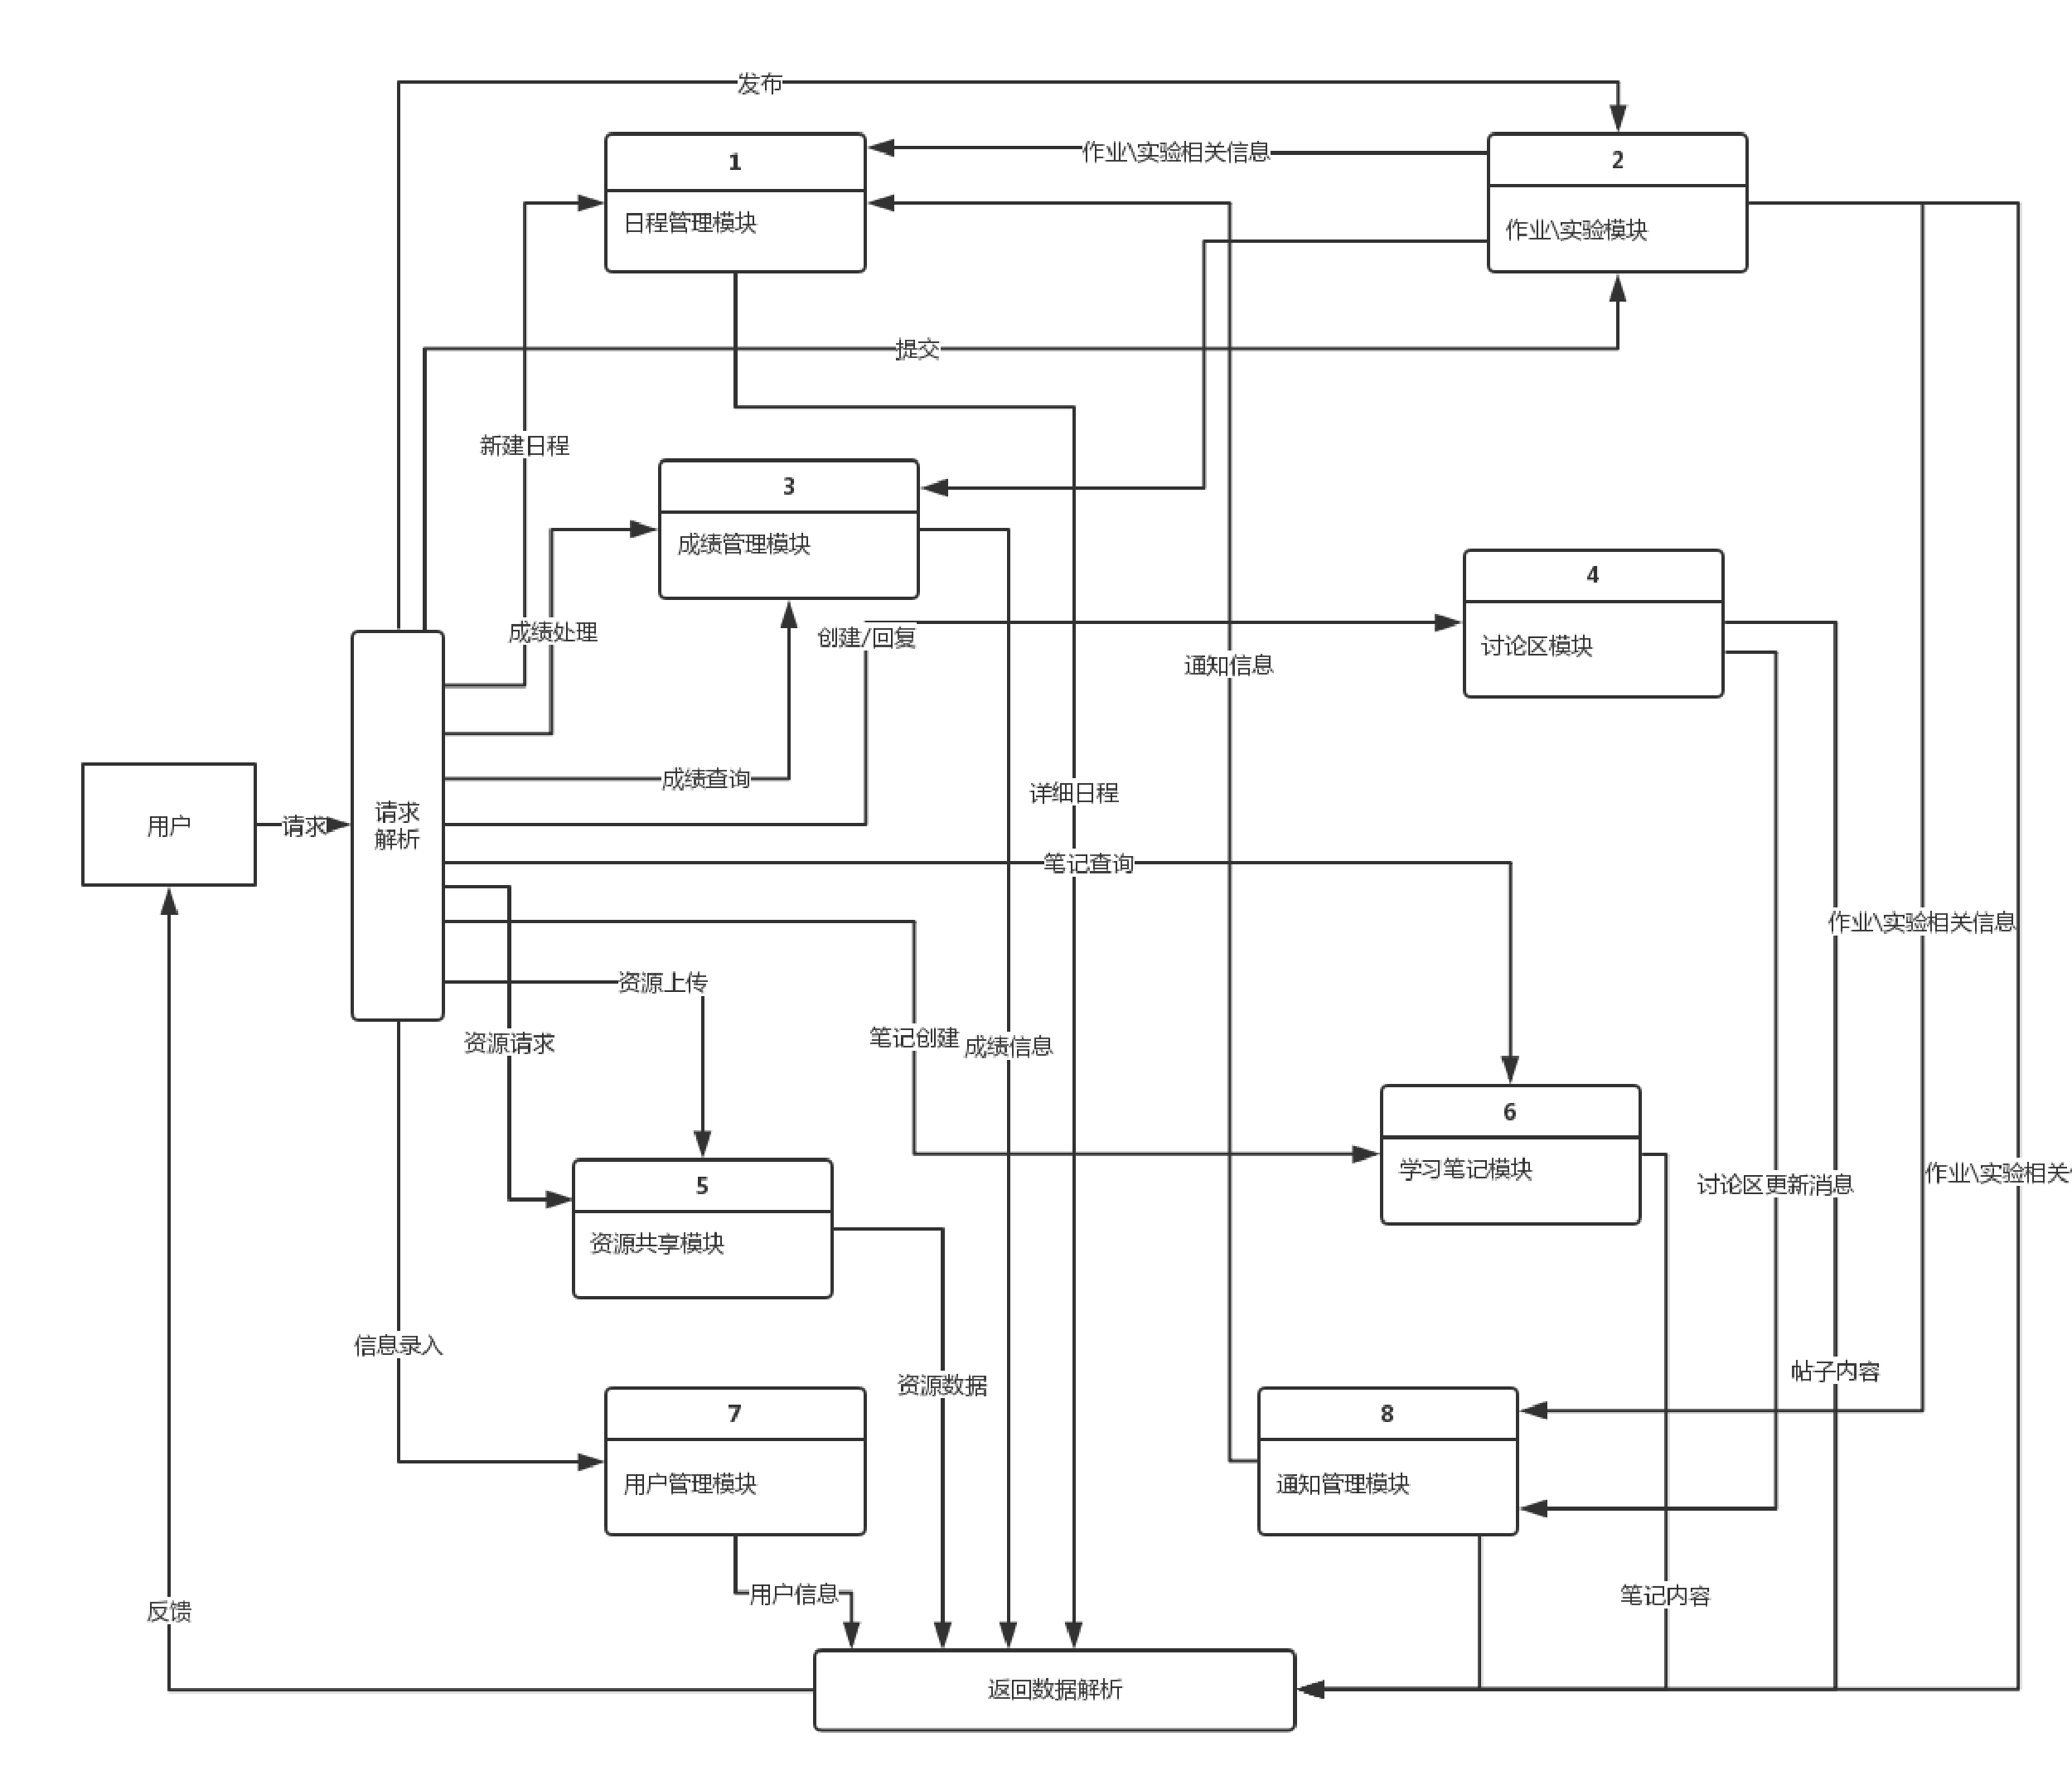
\includegraphics[width=15cm]{Level_0}
\caption{总体流程}
\end{figure}

\subsection{系统基本流程}
\subsubsection{日程管理模块}
\begin{figure}[H]
\centering
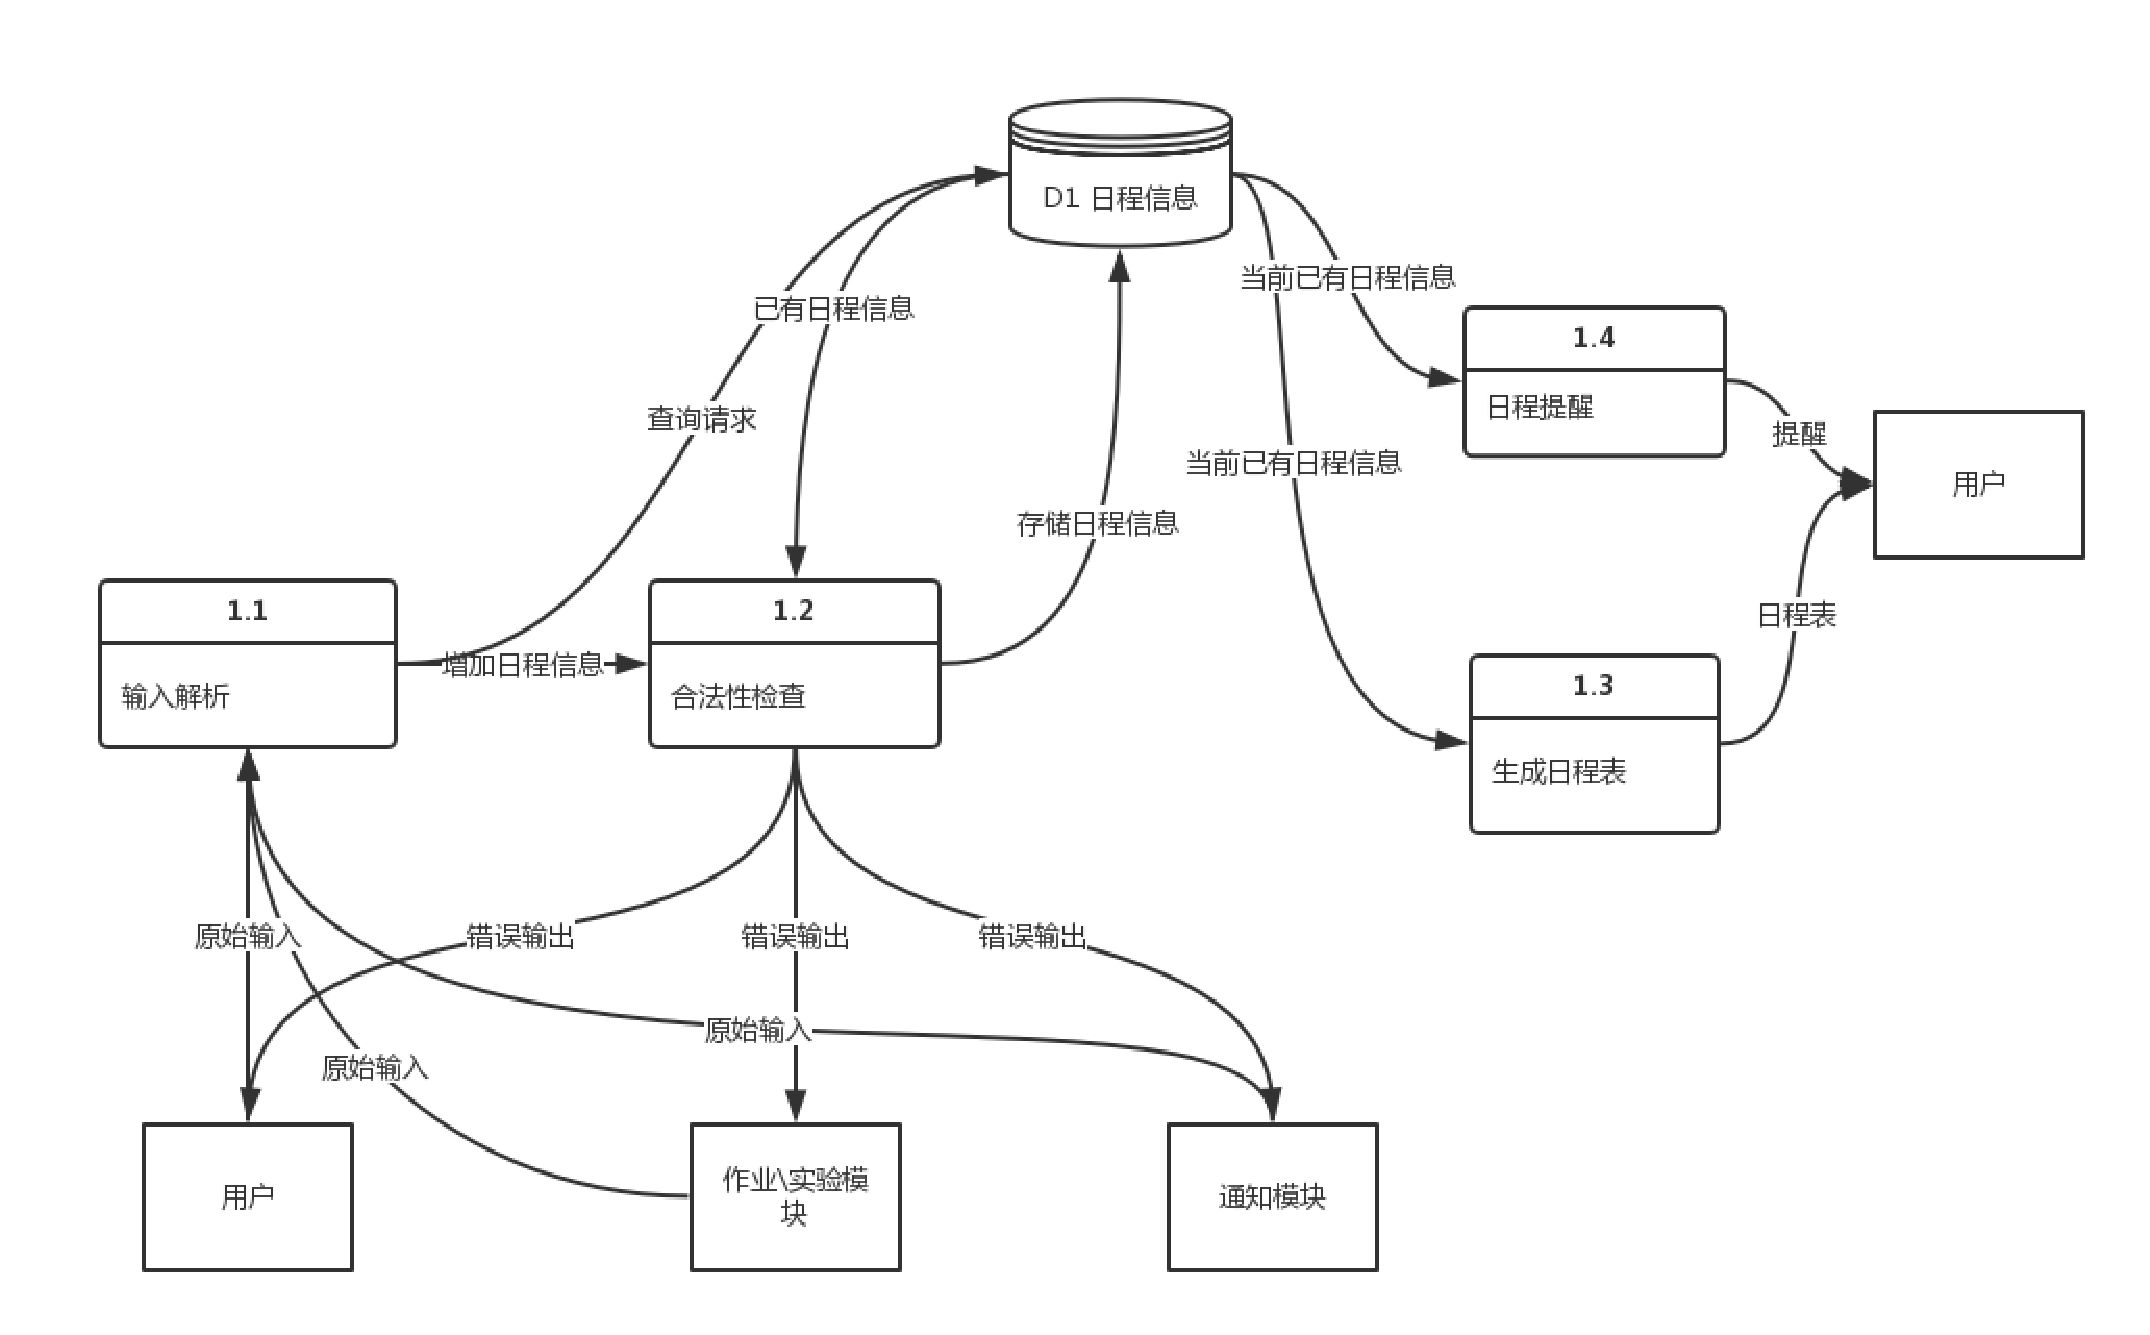
\includegraphics[width=15cm]{level1_1}
\caption{日程管理模块流程}
\end{figure}
\subsubsection{作业实验模块}
\begin{figure}[H]
\centering
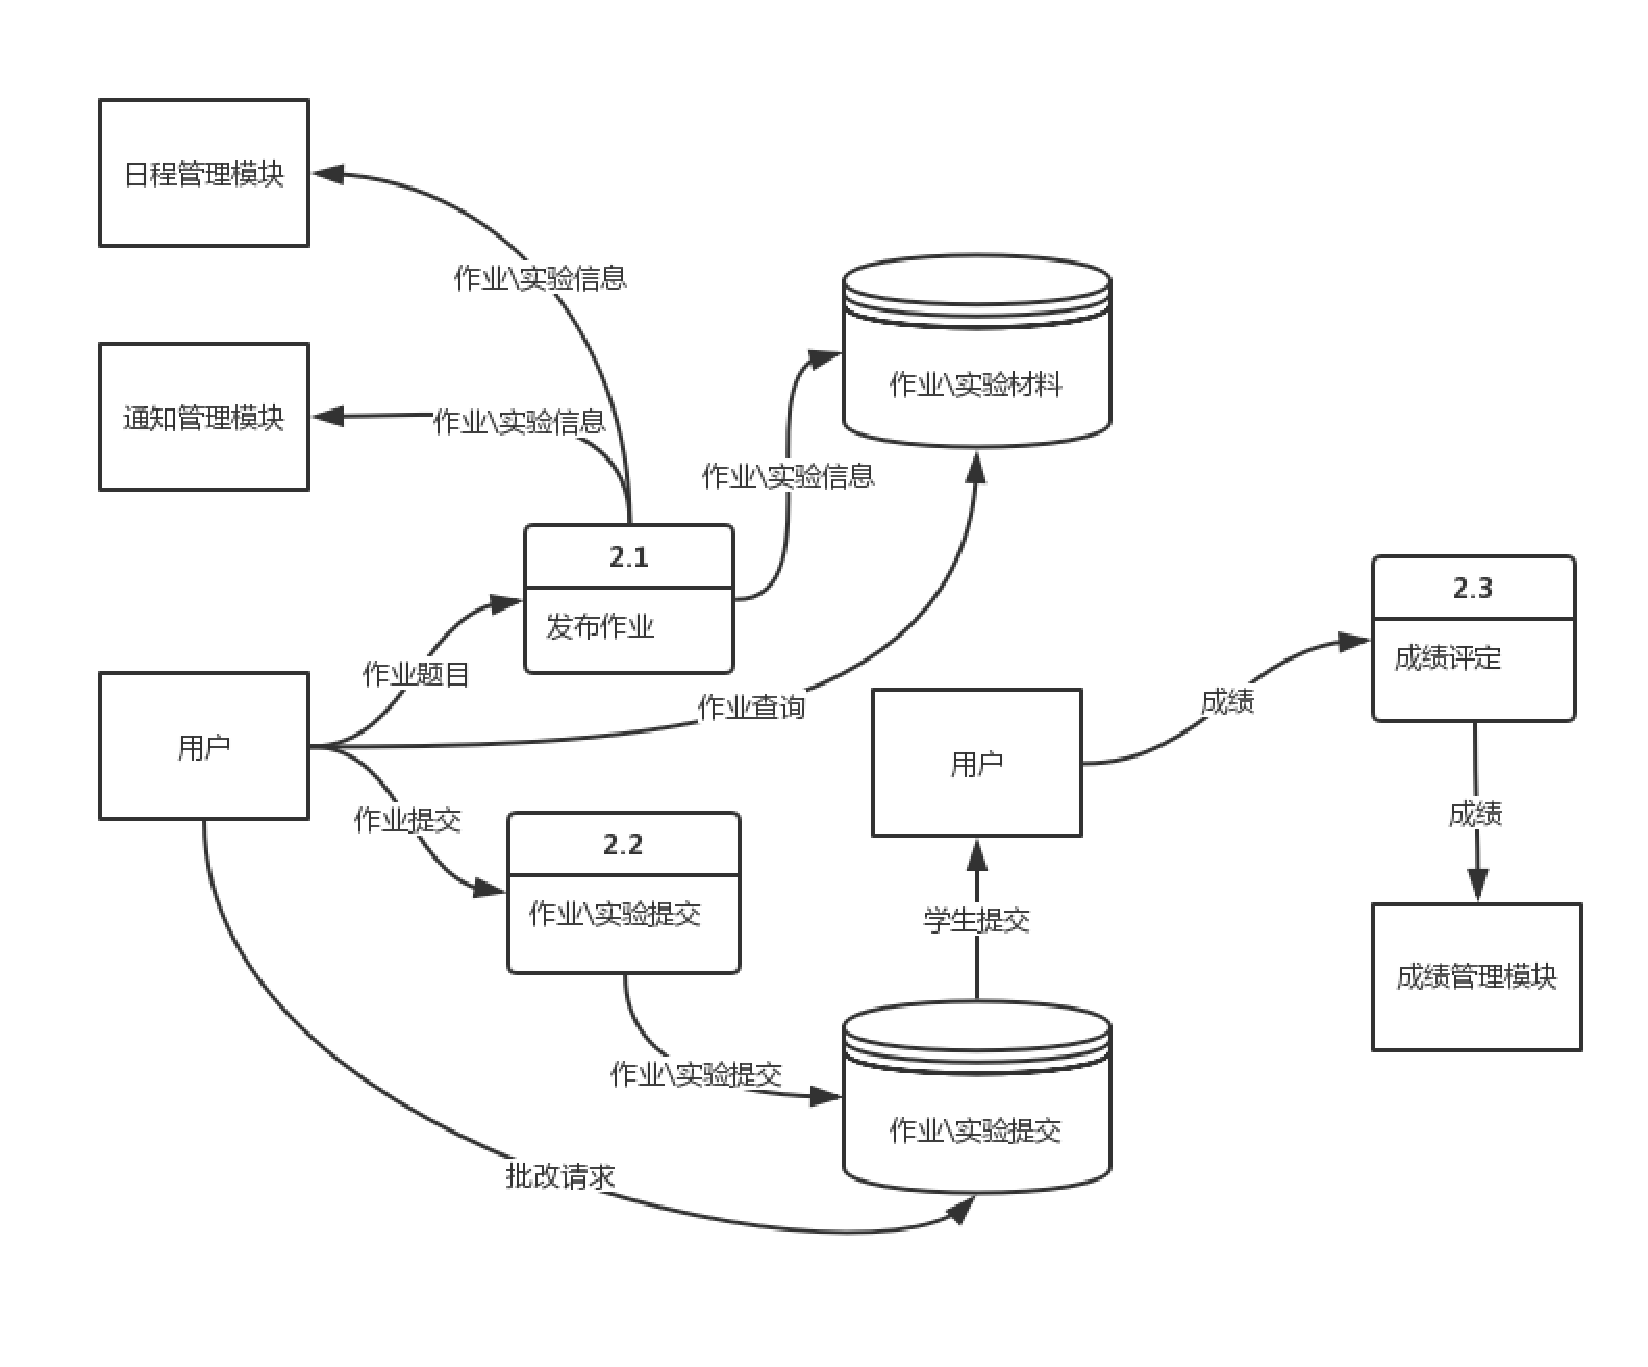
\includegraphics[width=15cm]{level1_2}
\caption{日程管理模块流程}
\end{figure}
\subsubsection{学习笔记模块}
\begin{figure}[H]
\centering
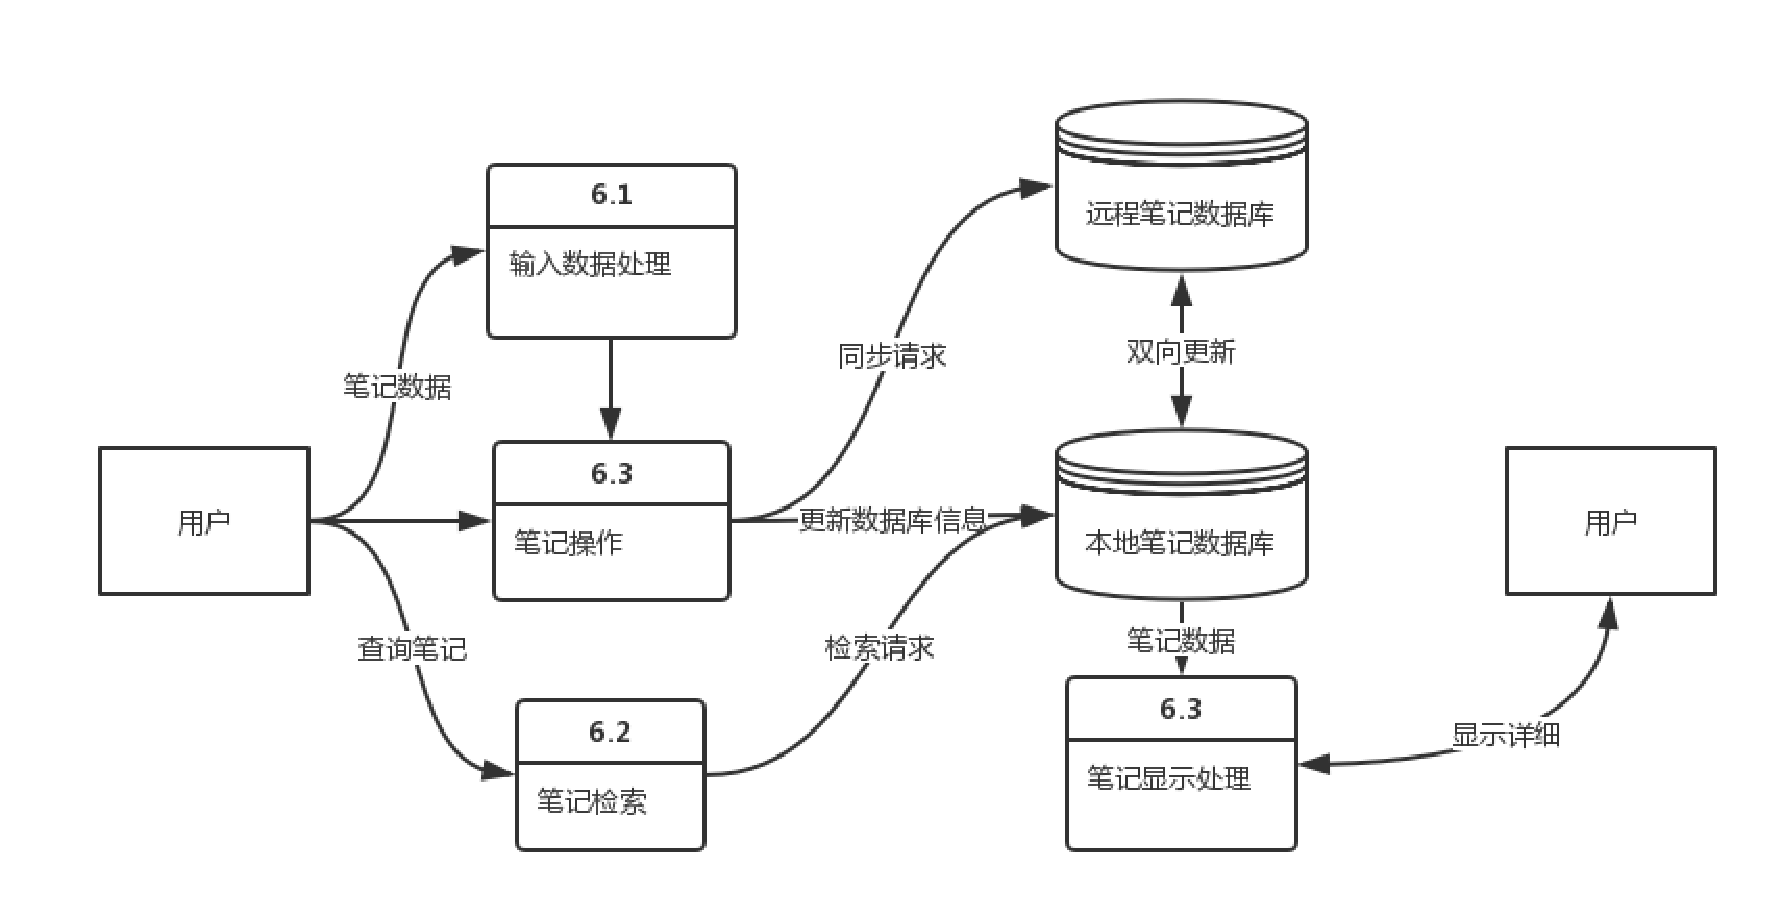
\includegraphics[width=15cm]{level1_3}
\caption{学习笔记模块流程}
\end{figure}
\subsubsection{成绩管理模块}
\begin{figure}[H]
\centering
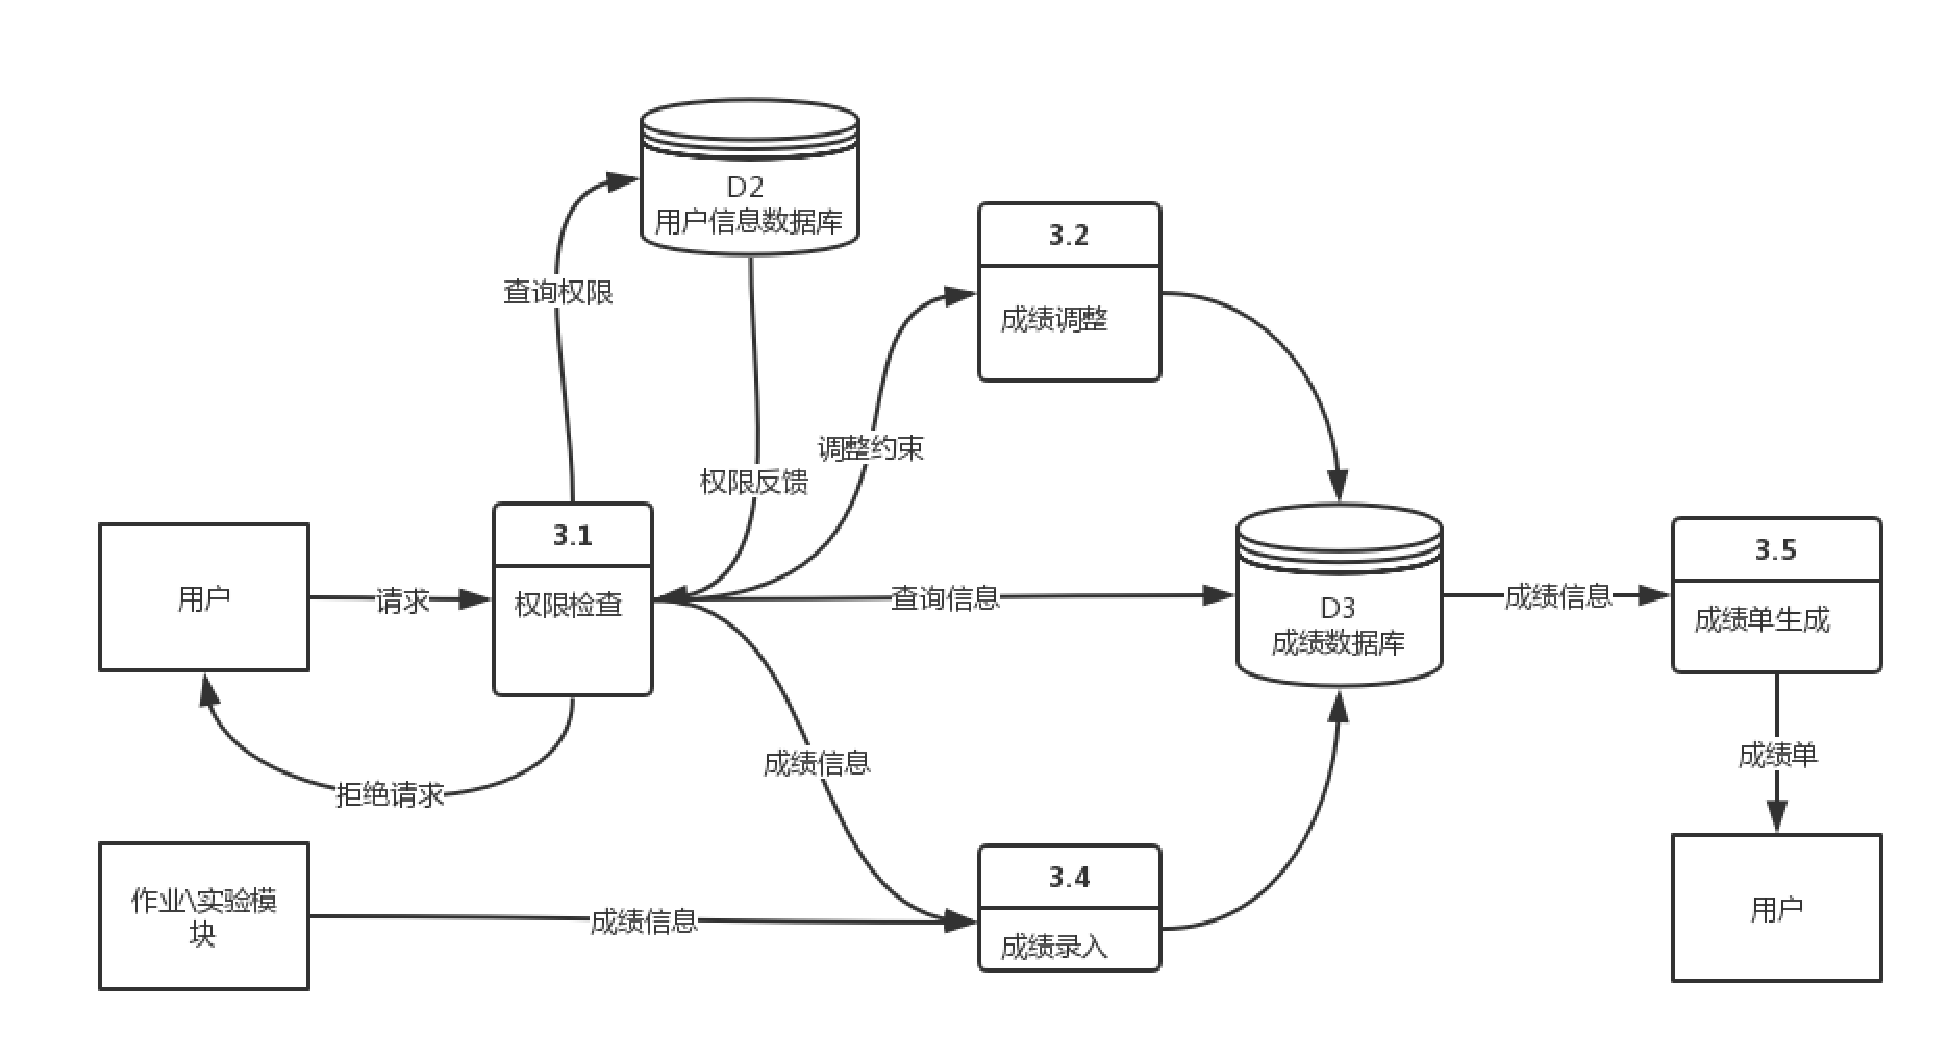
\includegraphics[width=15cm]{level1_4}
\caption{成绩管理模块流程}
\end{figure}
\subsubsection{用户管理模块}
\begin{figure}[H]
\centering
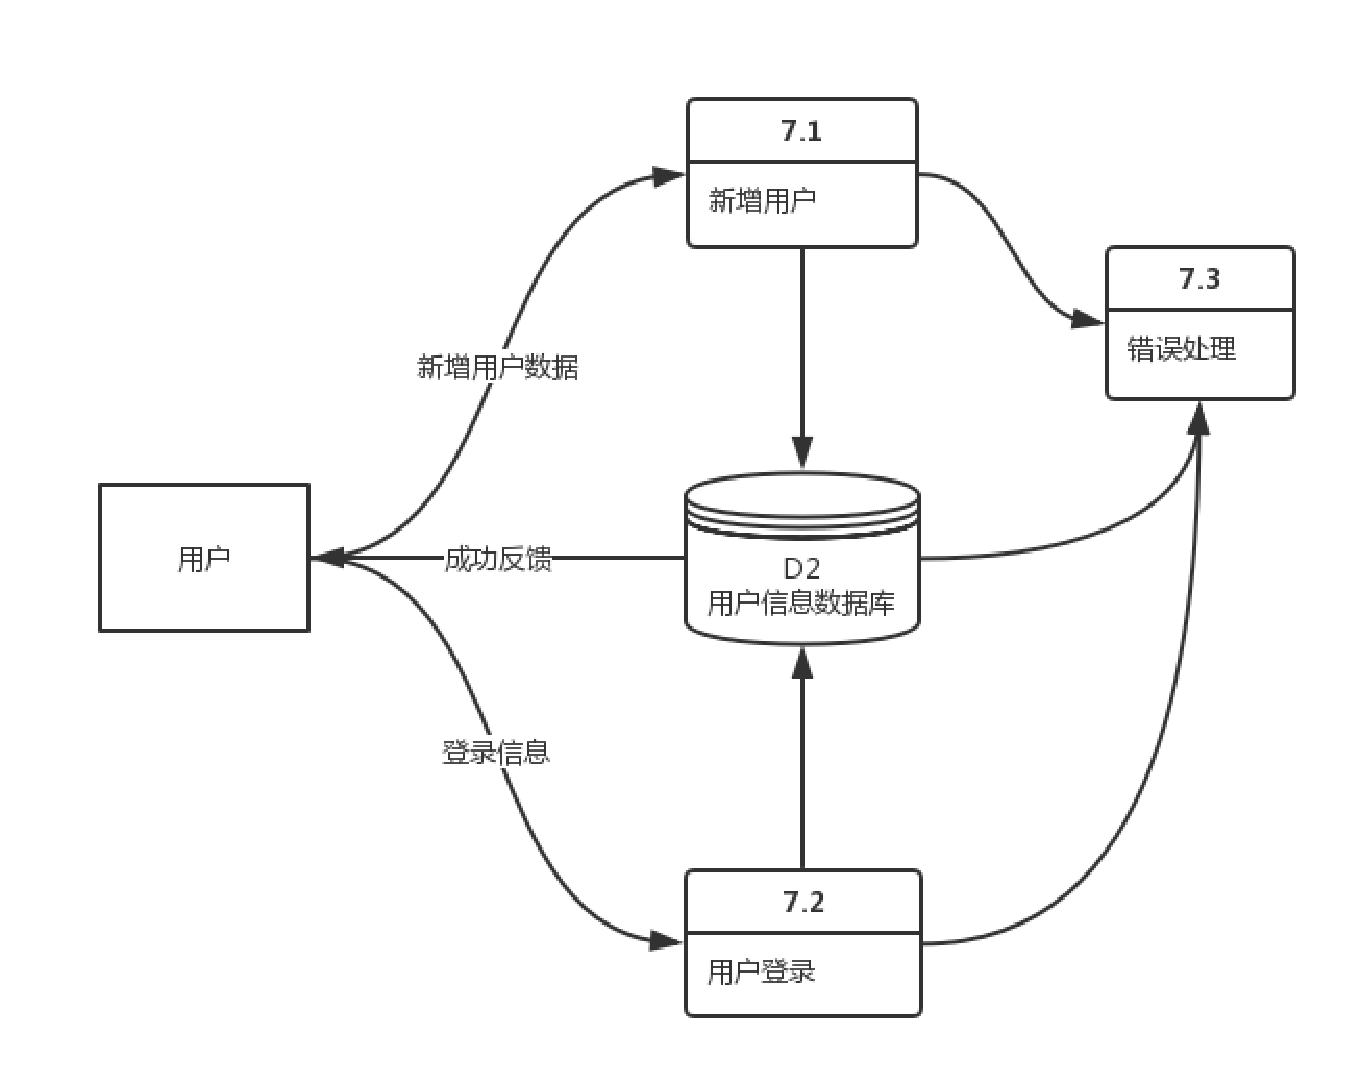
\includegraphics[width=15cm]{level1_5}
\caption{用户理模块流程}
\end{figure}
\subsubsection{讨论区模块}
\begin{figure}[H]
\centering
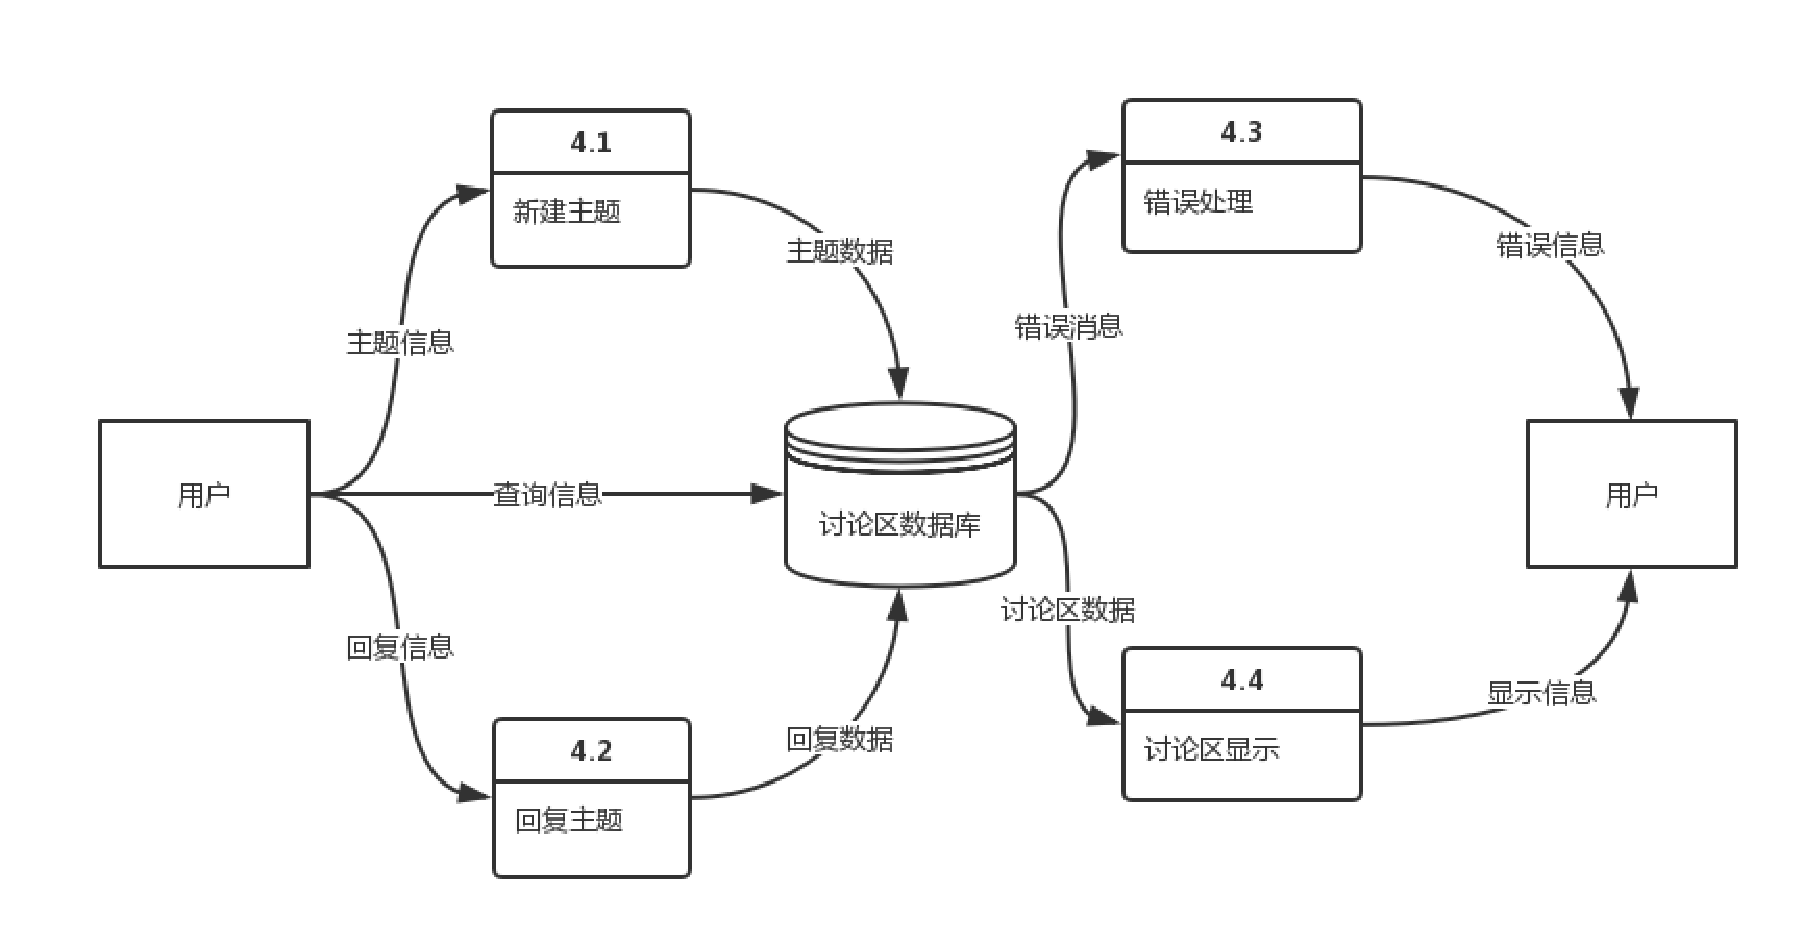
\includegraphics[width=15cm]{level1_6}
\caption{讨论区模块流程}
\end{figure}
\subsubsection{资源共享模块}
\begin{figure}[H]
\centering
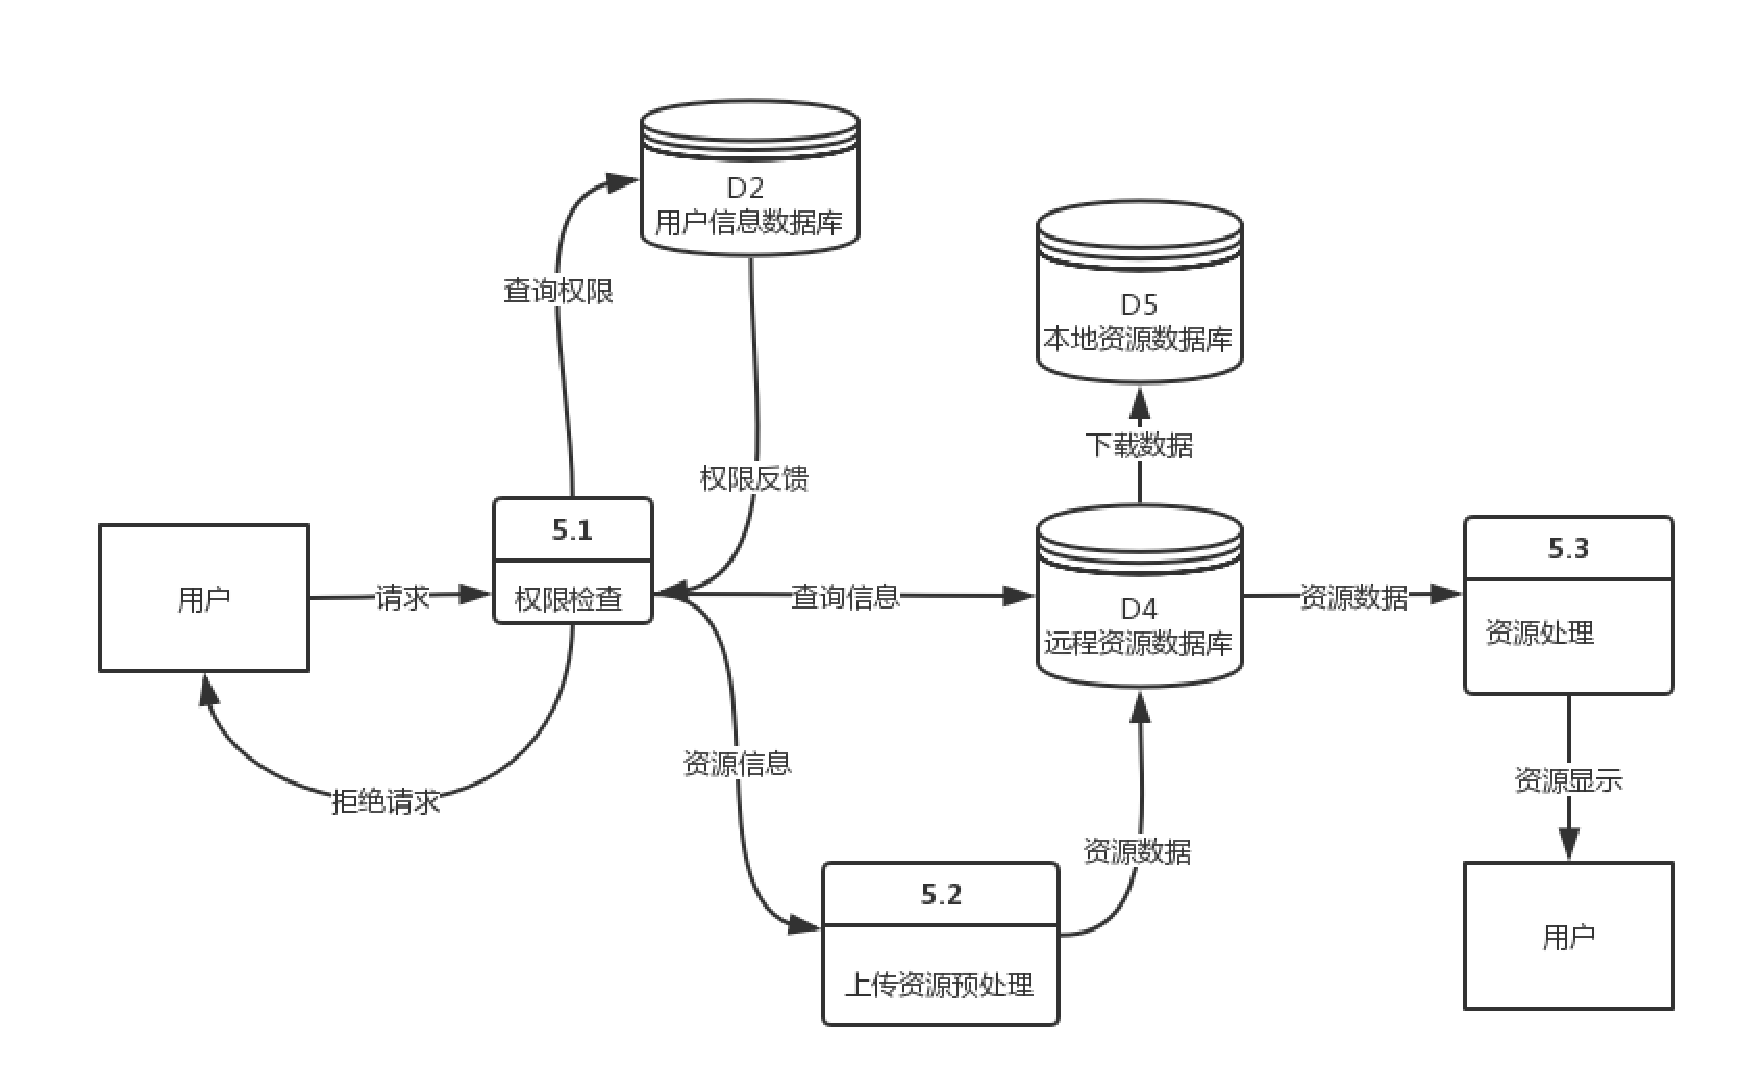
\includegraphics[width=15cm]{level1_7}
\caption{资源共享模块流程}
\end{figure}
\subsubsection{通知管理模块}
\begin{figure}[H]
\centering
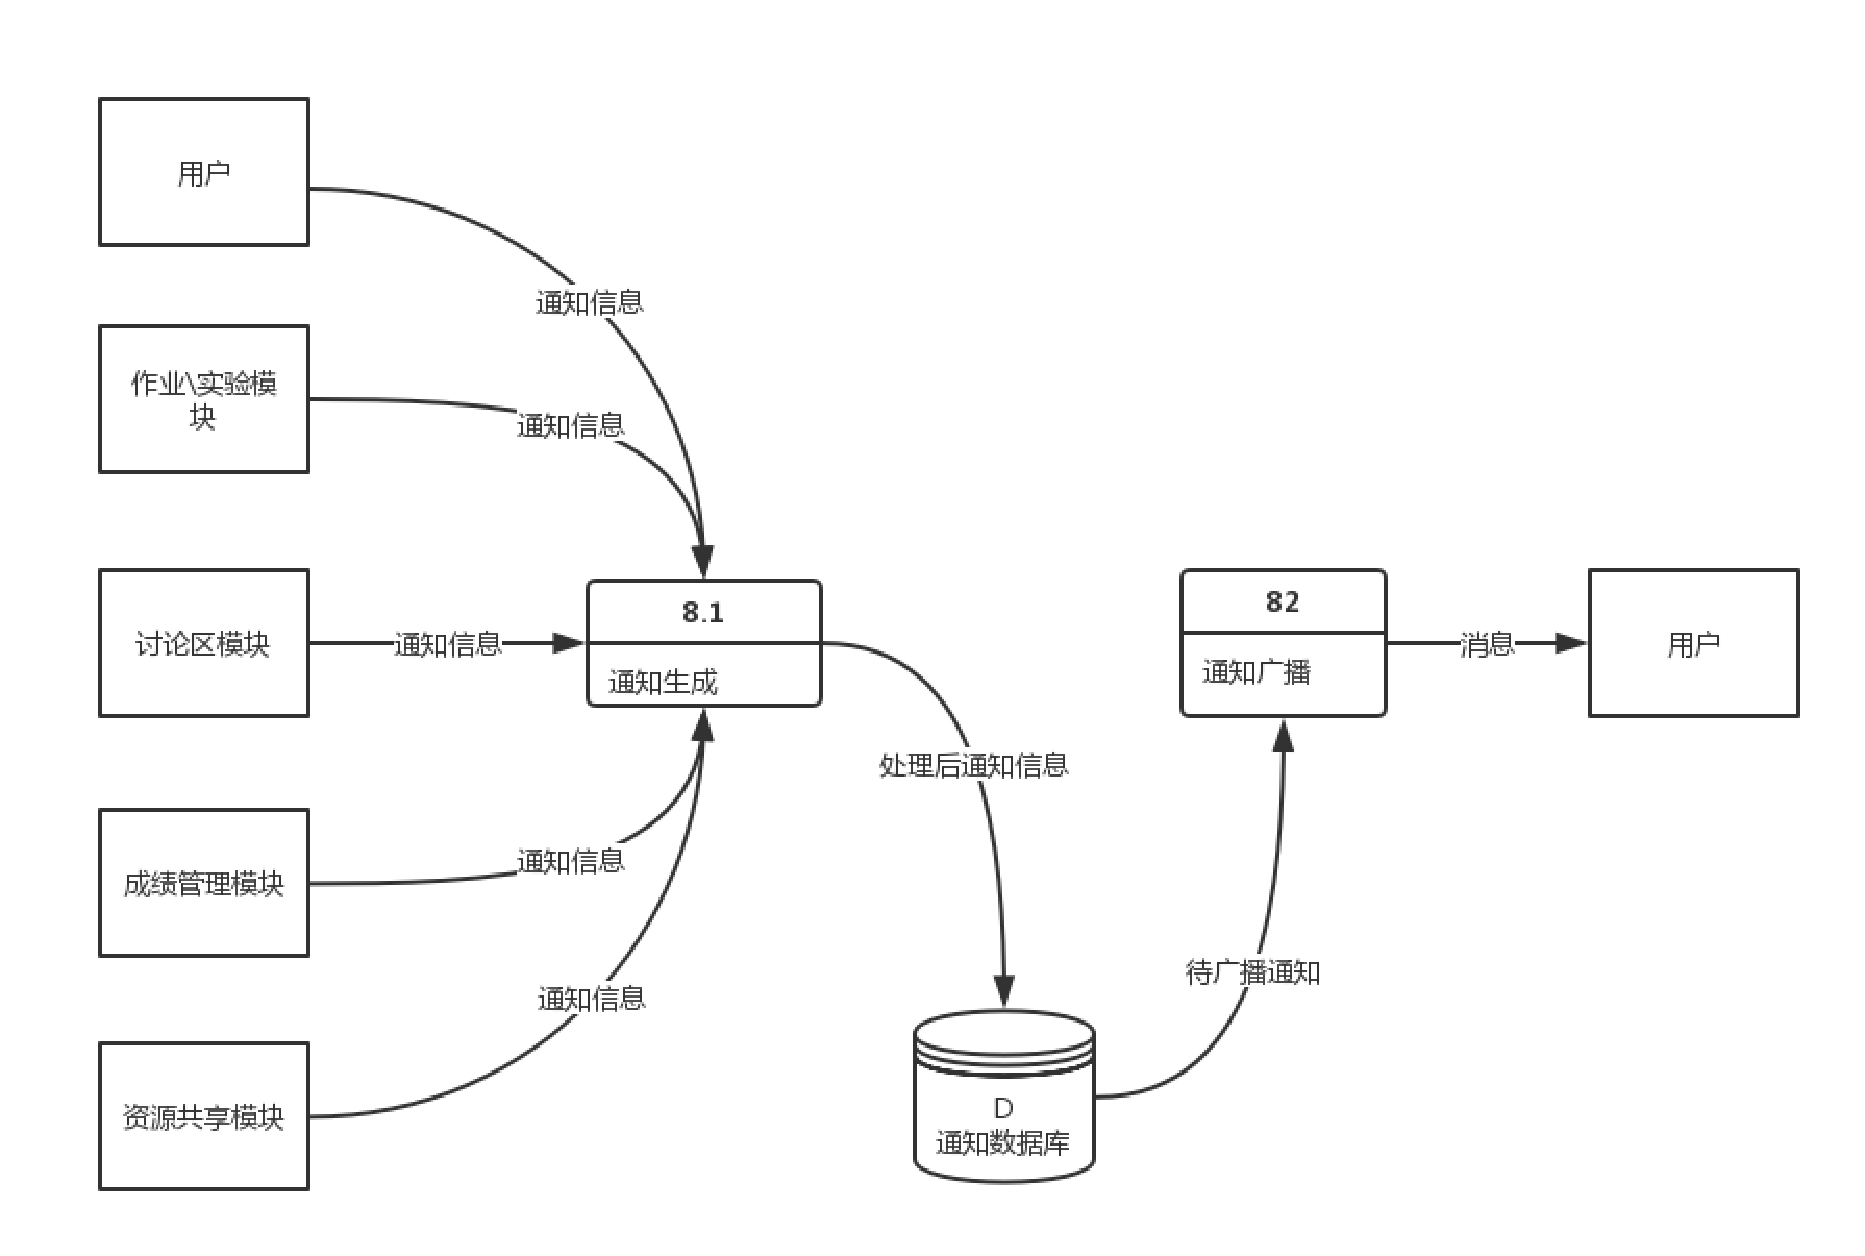
\includegraphics[width=15cm]{level1_8}
\caption{通知管理模块流程}
\end{figure}

\subsection{R.FUNC.BB.001   用户登陆}
客户端发送查询请求到服务器用户数据库,匹配该用户邮箱或学号和密码,匹配成功则返回成功登录的信息,并同步数据,进入登录后页面。匹配失败则返回失败信息,并显示账户不存在或密码错误。若为新用户,客户端发送新建请求到服务器数据库,检查是否为新用户,若可创建则返回允许创建信息,失败则返回无法创建新用户。

\subsection{R.FUNC.BB.002   作业/实验查询}
已登录用户在作业实验模块中提交查询请求,提交的表单中指明查找的关键字,由客户端和服务器端从本地存储和服务器存储的的数据文件进行搜索,对于符合关键字的搜索结果返回给用户,如果没有结果则显示无结果。

\subsection{R.FUNC.BB.003   作业/实验/通知发布}
教师在客户端作业实验端编辑要发布的信息的内容,并包括截止日期,附件等信息,上传到服务器,服务器判断用户发来的数据,将附件存入相应空间,将其他内容存入数据库中。再由服务器端向相应课程的学生客户端发出更新请求,更新日程和作业实验页面。

\subsection{R.FUNC.BB.004   作业/实验/通知修改删除}
教师通过客户端删除通知后,客户端删除本地缓存文件,同时在全局标签文件中删除信息,搜索日程中对应的作业实验并删除。编辑结束后上传删除信息,服务器进行相同的处理,并广播给相应课程的学生客户端,发出删除通知。

\subsection{R.FUNC.BB.005   作业/实验/通知提交}
学生将作业/实验内容从本地提交。服务器接受消息,更新数据库,并将收到的文件存储,向客户端发送结果信息。

\subsection{R.FUNC.BB.006   作业/实验查看与批改}
教师向服务器发出请求,下载班内同学作业到本地,或者在线浏览,批改,之后将批改结果上传到服务器端的相应位置,更新数据库中作业批改的信息,和相应课程同学的作业成绩。

\subsection{R.FUNC.BB.007   成绩录入}
教师通过客户端将学生成绩上传到服务器端的相应位置,更新数据库中作业或者考试信息,和相应课程同学的作业成绩,根据用户或者其他模块的输入构造满足后台数据存储结构的信息并且存储。服务器向学生端发送数据,包括课程成绩,教师的批改情况等信息。

\subsection{R.FUNC.BB.008   成绩查询}
学生通过客户端发送请求,包括课程信息等,服务器端在成绩统计系统中查找学生的课程成绩或作业成绩,将信息发送给客户端,并更新数据。

\subsection{R.FUNC.BB.009   成绩统计和调整}
教师端通过客户端查看学生成绩,并进行调整,服务器解析用户的调整需求看是否合法,如果合法则对数据库进行更新。

\subsection{R.FUNC.BB.0010   资源上传}
首先检查上传数据是否有效合法。不合法或者失效给出警告。合法则计算MD5查询数据库中是否已经存在相同资源,存在则只建立相应的链接,不存在则上传文件至远程数据库。

\subsection{R.FUNC.BB.0012   资源下载与浏览}
用户从服务器端获取数据,根据数据格式以及用户平台进行相应的转码处理最后交付客户端直接进行显示。

\subsection{R.FUNC.BB.0013   新建日程}
学生通过客户端编辑日程信息并提交,服务器端检查用户提供信息是否合法。日程的输入有多种格式,如果用户输入的不是标准的各项信息,而是纯文本等等,则首先尝试从中解析出事件地点描述等关键信息,尝试构建日程,成功则存入数据库,失败返回报错。成功后在日程管理系统中讲日程信息存入数据库,操作成功则返回成功信息到客户端。

\subsection{R.FUNC.BB.0014   日程显示与提醒}
客户端按设定频率检索当前日程数据库中的相关信息,比较当前日期,如果有满足提醒条件的则给用户发送提醒。

\subsection{R.FUNC.BB.0015   讨论区讨论}
用户在讨论区模块发送新建回复等请求,服务器端检查用户提供信息是否合法,然后将回复内容存入数据库中。客户端再从数据库中获取相关信息,处理渲染之后显示。

\subsection{R.FUNC.BB.0016   新建博文}
用户从讨论区模块创建新的博文,并在文本编辑器中编辑好文章,创建成功则将新的文章按用户选择存入本地存储,或存入服务器,并设定其他用户的浏览权限。

\subsection{R.FUNC.BB.0018   学习笔记文本添加}
用户从笔模块创建新的笔记,并在文本编辑器中编辑好文章,创建成功则将新的笔记按用户选择存入本地存储,或存入服务器,并设定其他用户的浏览权限。服务器检查用户提供信息是否合法。然后将其中的图片公式等等转换格式存入数据库中。

\section{功能结构设计}
\subsection{整体结构}

\begin{longtable}{| c | c | p{7cm} |}
% 首页表头
\caption[]{整体结构} \label{tab:longtable} \\
\toprule[1.5pt]
模块编号 & 模块名称 & 子功能结构\\
\midrule[1pt]
\endfirsthead
% 续页表头
\caption[]{整体结构(续)} \\
\toprule[1.5pt]
模块编号 & 模块名称 & 子功能结构\\
\midrule[1pt]
\endhead
% 首页表尾
\hline
\multicolumn{3}{r}{\small 续下页}
\endfoot
% 续页表尾
\bottomrule[1.5pt]
\endlastfoot
M.MODULE.BB.001   &   日程管理模块   &   日程管理功能结构   \\
    &   &   日程查询功能结构    \\
    &   &   新建日程功能结构    \\
    &   &   日程显示功能结构    \\

M.MODULE.BB.002   &   作业实验模块   &   作业实验功能结构   \\
    &   &   作业实验查询功能结构  \\
    &   &   新建作业功能结构    \\
    &   &   修改与删除作业功能结构 \\
    &   &   作业实验提交功能结构  \\

M.MODULE.BB.003   &   成绩管理模块   &   成绩管理功能结构   \\
    &   &   成绩查询功能结构    \\
    &   &   成绩导入功能结构    \\
    &   &   成绩调整功能结构    \\

M.MODULE.BB.004   &   讨论区模块   &   讨论区功能结构   \\
    &   &   发布主题功能结构    \\
    &   &   讨论区查询功能结构   \\
    &   &   修改与删除主题功能结构 \\

M.MODULE.BB.005   &   资源共享模块  &   资源共享功能结构   \\
    &   &   资源查询功能结构    \\
    &   &   资源上传功能结构    \\
    &   &   资源下载功能结构    \\

M.MODULE.BB.006   &   学习笔记模块   &   学习笔记功能结构   \\
    &   &   笔记上传功能结构    \\
    &   &   笔记查询功能结构    \\
    &   &   笔记修改与删除功能结构 \\

M.MODULE.BB.007   &   用户管理模块   &   用户管理功能结构   \\
    &   &   登录请求功能结构    \\

M.MODULE.BB.008   &   通知管理模块   &   通知管理功能结构   \\

\end{longtable}


\begin{figure}[H]
\centering
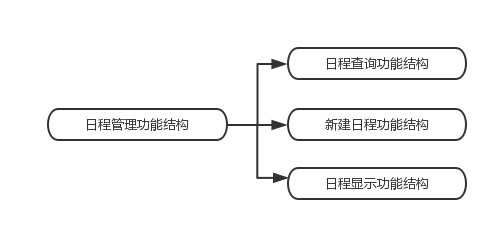
\includegraphics[width=15cm]{figu1}
\caption{日程管理功能结构}
\end{figure}

\begin{figure}[H]
\centering
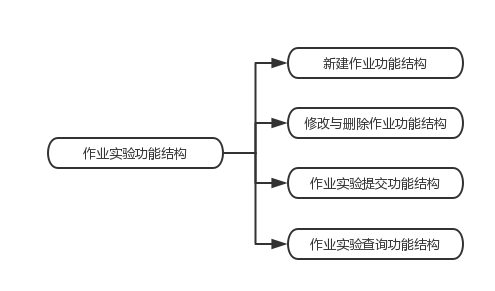
\includegraphics[width=15cm]{figure2}
\caption{作业实验功能结构}
\end{figure}

\begin{figure}[H]
\centering
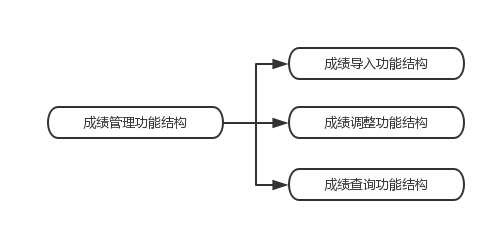
\includegraphics[width=15cm]{figu3}
\caption{成绩管理功能结构}
\end{figure}

\begin{figure}[H]
\centering
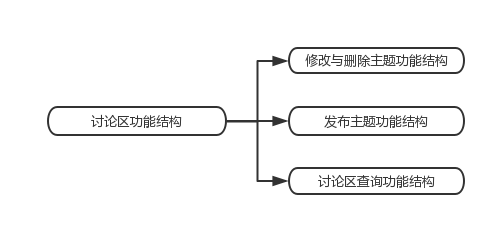
\includegraphics[width=15cm]{figu4}
\caption{讨论区功能结构}
\end{figure}

\begin{figure}[H]
\centering
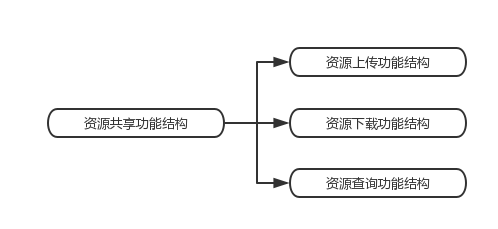
\includegraphics[width=15cm]{figu5}
\caption{资源共享功能结构}
\end{figure}

\begin{figure}[H]
\centering
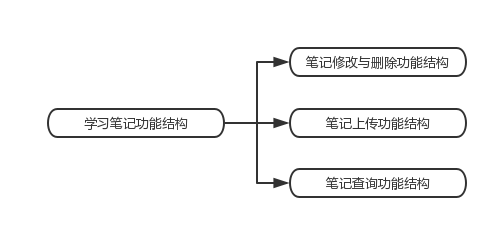
\includegraphics[width=15cm]{figu6}
\caption{学习笔记功能结构}
\end{figure}

\begin{figure}[H]
\centering
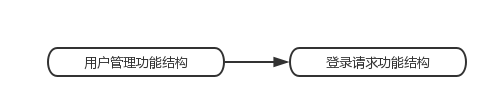
\includegraphics[width=15cm]{figu7}
\caption{用户管理功能结构}
\end{figure}

\subsection{用户与服务器功能结构}

客户端和服务器端的功能结构具体描述。

\subsubsection{MODULE.BB.001    日程管理功能结构}
提供日程管理的功能部件,本功能结构实现对编辑按钮、查询按钮、导出按钮、删除选项、已完成选项的布局和接口实现。
\\子功能结构:
\\MODULE.BB.015 日程查询功能结构
\\MODULE.BB.018 新建日程功能结构
\\MODULE.BB.019 日程显示功能结构

\subsubsection{MODULE.BB.002    作业实验功能结构}
提供作业实验的功能部件,本功能结构实现对编辑按钮、查询按钮、下载按钮、导出按钮、删除选项、已完成选项的布局和接口实现。
\\子功能结构:
\\MODULE.BB.020 新建作业功能结构
\\MODULE.BB.021 修改与删除作业功能结构
\\MODULE.BB.022 作业实验提交功能结构
\\MODULE.BB.009 作业实验查询功能结构

\subsubsection{MODULE.BB.003    成绩管理功能结构}
提供成绩管理的功能部件,本功能结构实现对查询成绩按钮、上传成绩按钮、已完成选项的布局和接口实现。
\\子功能结构:
\\MODULE.BB.023 成绩导入功能结构
\\MODULE.BB.024 成绩调整功能结构
\\MODULE.BB.010 成绩查询功能结构


\subsubsection{MODULE.BB.004    讨论区功能结构}
提供讨论区的功能部件,本功能结构实现对新建主题按钮、编辑主题按钮、查询按钮、上传按钮、删除选项、已完成选项的布局和接口实现。
\\子功能结构:
\\MODULE.BB.025 修改与删除主题功能结构
\\MODULE.BB.016 发布主题功能结构
\\MODULE.BB.011 讨论区查询功能结构

\subsubsection{MODULE.BB.005    资源共享功能结构}
提供成绩的功能部件,本功能结构实现对编辑按钮、查询按钮、下载选项、上传选项、删除选项、已完成选项的布局和接口实现。
\\子功能结构:
\\MODULE.BB.026 资源上传功能结构
\\MODULE.BB.028 资源下载功能结构
\\MODULE.BB.012 资源查询功能结构

\subsubsection{MODULE.BB.006    学习笔记功能结构}
提供成绩的功能部件,本功能结构实现对编辑按钮、查询按钮、上传按钮、下载按钮、在线浏览、删除选项、已完成选项的布局和接口实现。
\\子功能结构:
\\MODULE.BB.017 笔记上传功能结构
\\MODULE.BB.013 笔记查询功能结构
\\MODULE.BB.027 笔记修改与删除功能结构

\subsubsection{MODULE.BB.007    用户管理功能结构}
服务器端提供用户信息管理的功能部件,本功能结构实现对用户信息的导入,查询,删除,编辑、已完成选项的布局和接口实现。
\\子功能结构:
\\MODULE.BB.014 登录请求功能结构

\subsubsection{MODULE.BB.008    通知管理功能结构}
根据本地数据库查询找到需要提醒的时间,实现一个 Android Fragment 用于时间的设置并触发一个 Thread 用于该提醒的计时。

\subsubsection{MODULE.BB.009    作业实验查询功能结构}
作业实验查询功能由触发查询按钮的回调函数实现,本功能结构完成对查询关键字的 分词、分析和转化,并完成查询和分类展示的部分。

\subsubsection{MODULE.BB.010    成绩查询管理功能结构}
成绩查询功能由触发查询按钮的回调函数实现,本功能结构完成对查询关键字的 分词、分析和转化,并完成查询和分类展示的部分。

\subsubsection{MODULE.BB.011    讨论区查询功能结构}
讨论区查询功能由触发查询按钮的回调函数实现,本功能结构完成对查询关键字的 分词、分析和转化,并完成查询和分类展示的部分。

\subsubsection{MODULE.BB.012    资源查询功能结构}
资源查询功能由触发查询按钮的回调函数实现,本功能结构完成对查询关键字的 分词、分析和转化,并完成查询和分类展示的部分。

\subsubsection{MODULE.BB.013    笔记查询功能结构}
笔记查询功能由触发查询按钮的回调函数实现,本功能结构完成对查询关键字的 分词、分析和转化,并完成查询和分类展示的部分。

\subsubsection{MODULE.BB.014    登录请求功能结构}
登录界面由一个 Android Activity 实现,并用 socket 的方式连接服务器确认登录情况。

\subsubsection{MODULE.BB.015    日程查询功能结构}
日程查询功能由触发查询按钮的回调函数实现,本功能结构完成对查询关键字的 分词、分析和转化,并完成查询和分类展示的部分。

\subsubsection{MODULE.BB.016    发布主题功能结构}
布局在 note.xml 布局文件中实现。完成编辑界面的布局。编辑界面作为一个 新的 Android Activity 实现。
编辑界面完成文本编辑功能,并为添加图片、添加画图、添加书签的实现准 备好接口。
实现基本的时间记录功能,编辑结束后,笔记内容以 xml 的格式保存在本地 APP 文件下,每次客户端打开时读取 xml 文件并解析。

\subsubsection{MODULE.BB.017    笔记上传功能结构}
MODULE.BB.006    学习笔记功能结构后用户选择是否调用该功能结构,实现笔记的上传功能。

\subsubsection{MODULE.BB.018    新建日程功能结构}
布局在 note.xml 布局文件中实现。完成编辑界面的布局。编辑界面作为一个 新的 Android Activity 实现。
编辑界面完成文本编辑功能,并为添加图片、添加画图、添加书签的实现准 备好接口。
实现基本的时间记录功能,编辑结束后,日程内容以 xml 的格式保存在本地 APP 文件下,每次日程打开时读取 xml 文件并解析。

\subsubsection{MODULE.BB.019    日程显示功能结构}
本功能结构由一个 Android Fragment 实现结果的分类展示。

\subsubsection{MODULE.BB.020    新建作业功能结构}
布局在 note.xml 布局文件中实现。完成编辑界面的布局。编辑界面作为一个 新的 Android Activity 实现。
编辑界面完成文本编辑功能,并为添加图片、添加画图、添加书签的实现准 备好接口。
实现基本的时间记录功能,编辑结束后,作业内容以 xml 的格式保存在本地 APP 文件下,每次作业实验模块打开时读取 xml 文件并解析。

\subsubsection{MODULE.BB.021    修改与删除作业功能结构}
完成编辑和删除作业功能,编辑结束后,作业内容以 xml 的格式保存在本地 APP 文件下,每次作业实验模块打开时读取 xml 文件并解析。

\subsubsection{MODULE.BB.022    作业实验提交功能结构}
从本地资源管理器中选择要提交的作业实验文件上传到数据库中。

\subsubsection{MODULE.BB.023    成绩导入功能结构}
教师调用该功能结构,实现成绩的上传功能。

\subsubsection{MODULE.BB.024    成绩调整功能结构}
界面在.xml文件中实现,并可在线编辑文件。

\subsubsection{MODULE.BB.025    修改与删除主题功能结构}
完成编辑和删除作业功能,编辑结束后,作业内容以 xml 的格式保存在本地 APP 文件下,每次讨论区模块打开时读取 xml 文件并解析。

\subsubsection{MODULE.BB.026    资源上传功能结构}
用户选择调用该功能结构,实现课件等的上传功能。

\subsubsection{MODULE.BB.027    笔记修改与删除功能结构}
完成编辑和删除作业功能,编辑结束后,笔记内容以 xml 的格式保存在本地 APP 文件下,每次笔记模块打开时读取 xml 文件并解析。

\subsubsection{MODULE.BB.028    资源下载功能结构}
用户选择调用该功能结构,实现课件等的下载功能。


\section{功能需求与程序代码的关系}
[此处指的是不同的需求分配到哪些模块去实现。可按不同的端拆分此表]
\begin{longtable}{|c|c|c|c|}
% 首页表头
\caption[]{功能需求与程序代码的关系} \label{tab:longtable} \\
\toprule[1.5pt]
功能需求编号 & 功能需求 & 功能结构编号 & 功能结构 \\
\midrule[1pt]
\endfirsthead
% 续页表头
\caption[]{整体结构(续)} \\
\toprule[1.5pt]
功能需求编号 & 功能需求 & 功能结构编号 & 功能结构 \\
\midrule[1pt]
\endhead
% 首页表尾
\hline
\multicolumn{3}{r}{\small 续下页}
\endfoot
% 续页表尾
\bottomrule[1.5pt]
\endlastfoot
R.FUNC.BB.001   &   用户登陆   &    MODULE.BB.007  &  用户管理功能结构  \\
   &   &   MODULE.BB.014   &   登录请求功能结构  \\

R.FUNC.BB.002   &   作业/实验查询   &   MODULE.BB.002  &  作业实验功能结构   \\
    &   &   MODULE.BB.001   &   日程管理功能结构    \\
    &   &   MODULE.BB.009   &   作业实验查询功能结构  \\

R.FUNC.BB.003   &   作业/实验/通知发布   &   MODULE.BB.002  &  作业实验功能结构 \\
    &   &   MODULE.BB.020  &  新建作业功能结构    \\

R.FUNC.BB.004   &   作业/实验/通知修改删除   &   MODULE.BB.021   & 修改与删除作业功能结构  \\

R.FUNC.BB.005   &   作业/实验/通知提交   &   MODULE.BB.022  &  作业实验提交功能结构   \\

R.FUNC.BB.006   &   作业/实验查看与批改   &   MODULE.BB.002  &  作业实验功能结构   \\
    &   &   MODULE.BB.003   &   成绩管理功能结构     \\

R.FUNC.BB.007   &   成绩录入   &  MODULE.BB.023  &  成绩导入功能结构    \\

R.FUNC.BB.008   &   成绩查询   &   MODULE.BB.003   &   成绩管理功能结构     \\
    &   &   MODULE.BB.010   &   成绩查询管理功能结构  \\
    &   &   MODULE.BB.008   &   通知管理功能结构    \\

R.FUNC.BB.009   &   成绩统计和调整   &    MODULE.BB.003   &   成绩管理功能结构     \\
    &   &   MODULE.BB.010   &   成绩查询管理功能结构  \\
    &   &   MODULE.BB.002  &  作业实验功能结构  \\
    &   &   MODULE.BB.024   & 成绩调整功能结构  \\

R.FUNC.BB.010   &   资源上传   &    MODULE.BB.005   &   资源共享功能结构   \\
    &   &   MODULE.BB.026  &  资源上传功能结构  \\

R.FUNC.BB.012   &   资源下载与浏览   &   MODULE.BB.005   &   资源共享功能结构   \\
    &   &   MODULE.BB.012  &  资源查询功能结构  \\
    &   &   MODULE.BB.026  &  资源下载功能结构  \\

R.FUNC.BB.013   &   新建日程   &   MODULE.BB.018   &   新建日程功能结构   \\

R.FUNC.BB.014   &   日程显示与提醒   &   MODULE.BB.019  &  日程显示功能结构   \\
    &   &   MODULE.BB.008  &  通知管理功能结构 \\

R.FUNC.BB.015   &   讨论区讨论   &  MODULE.BB.004   & 讨论区功能结构   \\
    &   &   MODULE.BB.025  &  修改与删除主题功能结构\\

R.FUNC.BB.016   &   新建博文   &   MODULE.BB.004  &  讨论区功能结构   \\
    &   &   MODULE.BB.016  &  发布主题功能结构  \\

R.FUNC.BB.017   &   课程考试排布   &   MODULE.BB.001  &  日程管理功能结构   \\
    &   &   MODULE.BB.015  &  日程查询功能结构  \\

R.FUNC.BB.018   &   学习笔记文本添加   &   MODULE.BB.006  &  学习笔记功能结构    \\

R.FUNC.BB.019   &   学习笔记课件修改   &   MODULE.BB.027  &  笔记修改与删除功能结构   \\

R.FUNC.BB.020   &   学习笔记搜索   &   MODULE.BB.013  &  学习笔记查询功能结构   \\
    &   &   MODULE.BB.006  &  学习笔记功能结构    \\

R.FUNC.BB.021   &   学习笔记删除   &   MODULE.BB.027  &  笔记修改与删除功能结构   \\
    &   &   MODULE.BB.013  &  学习笔记查询功能结构   \\

R.FUNC.BB.022   &   学习笔记共享   &   MODULE.BB.006  &  学习笔记功能结构 \\
    &   &   MODULE.BB.013  &  学习笔记查询功能结构   \\
    &   &   MODULE.BB.017  &  笔记上传功能结构  \\



\end{longtable}
